% ----------------------------------------------------------------------------------------\
% ---------------------------------------------------------------------------------------\
% --------------------------------------------------------------------------------------\
\section{Instrucciones}
% ----------------------------------------------------------------------------------------\
% ---------------------------------------------------------------------------------------\
% --------------------------------------------------------------------------------------\

\begin{enumerate}
    \item \section{Implementación básica del Juego de la Vida}
    \subsection{Descripción del código}

El código implementa el Juego de la Vida, un autómata celular que simula el comportamiento de un sistema de células vivas y muertas en una cuadrícula, el código consta de las siguientes partes principales:

\subsection{Creación del estado inicial del juego}

La función \textbf{crear\_matriz\_inicial} genera una matriz cuadrada de tamaño $n \times n$ con valores aleatorios de 0 (célula muerta) y 1 (célula viva), esta matriz representa el estado inicial del juego.

\begin{lstlisting}
def crear_matriz_inicial(n):
    """
    Genera una matriz n x n con celulas vivas o muertas aleatoriamente.
    
    Parametros:
    - n: Tamano de la matriz (numero de filas y columnas).
    
    Retorna:
    - Matriz n x n con valores aleatorios 0 (muerta) o 1 (viva).
    """
    return np.random.choice([0, 1], size=(n, n))
\end{lstlisting}

\subsection{Aplicación de las reglas del Juego de la Vida}

La función \textbf{aplicar\_reglas} toma el estado actual del juego como entrada y aplica las reglas del Juego de la Vida para determinar el siguiente estado, las reglas son:
\begin{itemize}
    \item Una célula viva con dos o tres vecinas vivas sobrevive.
    \item Una célula muerta con tres vecinas vivas nace.
    \item En cualquier otro caso, la célula muere.
\end{itemize}

\begin{lstlisting}
def aplicar_reglas(estado_actual):
    """
    Aplica las reglas del Juego de la Vida a cada celula de la matriz.
    
    Parametros:
    - estado_actual: Matriz que representa el estado actual del juego.
    
    Retorna:
    - Nuevo estado del juego despues de aplicar las reglas.
    """
    n = estado_actual.shape[0]
    nuevo_estado = np.zeros((n, n))
    
    for i in range(n):
        for j in range(n):
            num_vecinos = np.sum(estado_actual[i-1:i+2, j-1:j+2]) - estado_actual[i, j]
            
            # Regla a) Si una celula esta viva y tiene dos o tres vecinas vivas, sobrevive.
            if estado_actual[i, j] == 1 and num_vecinos in [2, 3]:
                nuevo_estado[i, j] = 1
                        
            # Regla b) Si una celula esta muerta y tiene tres vecinas vivas, nace.
            elif estado_actual[i, j] == 0 and num_vecinos == 3:
                nuevo_estado[i, j] = 1
            else:
                nuevo_estado[i, j] = 0
    
    return nuevo_estado
\end{lstlisting}

\subsection{Visualización del estado del juego}

La función \textbf{visualizar\_estado} se utiliza para mostrar el estado actual del juego mediante una imagen en escala de grises.

\begin{lstlisting}
def visualizar_estado(estado, titulo="Estado del Juego de la Vida"):
    """
    Visualiza el estado del juego.
    
    Parametros:
    - estado: Matriz que representa el estado actual del juego.
    - titulo: Titulo para la visualizacion.
    """
    plt.figure(figsize=(5, 5))
    plt.imshow(estado, cmap='Greys', interpolation='nearest')
    plt.title(titulo)
    plt.show()
\end{lstlisting}

\subsection{Actualización de la matriz y visualización a través de múltiples turnos}

Esta sección del código implementa un bucle que actualiza la matriz basándose en las reglas y visualiza el estado de la cuadrícula después de cada actualización.

\begin{lstlisting}
# Numero de iteraciones/turnos para visualizar
num_iteraciones = 5
n = 10  # Tamano de la matriz

# Generar el estado inicial del juego
estado_actual = crear_matriz_inicial(n)

# Visualizar el estado inicial
visualizar_estado(estado_actual, "Estado Inicial")

# Bucle para actualizar y visualizar el juego en cada turno
for i in range(num_iteraciones):
    # Aplicar las reglas del Juego de la Vida para obtener el nuevo estado
    estado_actual = aplicar_reglas(estado_actual)
    # Visualizar el estado actual despues de aplicar las reglas
    visualizar_estado(estado_actual, titulo=f"Estado despues de {i + 1} turno(s)")
\end{lstlisting}



\subsection{Ejemplos}

A continuación se presentan dos casos diferentes de estados iniciales y se visualiza su evolución a través de 5 turnos.

\begin{itemize}
    \item Estado inicial aleatorio\\

   \begin{lstlisting}
# Número de iteraciones/turnos para visualizar
num_iteraciones = 5
n = 10  # Tamaño de la matriz

# Generar el estado inicial del juego
estado_actual = crear_matriz_inicial(n)

# Visualizar el estado inicial
visualizar_estado(estado_actual, "Estado Inicial")

# Bucle para actualizar y visualizar el juego en cada turno
for i in range(num_iteraciones):
    # Aplicar las reglas del Juego de la Vida para obtener el nuevo estado
    estado_actual = aplicar_reglas(estado_actual)
    # Visualizar el estado actual después de aplicar las reglas
    visualizar_estado(estado_actual, titulo=f"Estado después de {i + 1} turno(s)")
\end{lstlisting}

Los estados se muestran de la siguiente forma:
\begin{center}
    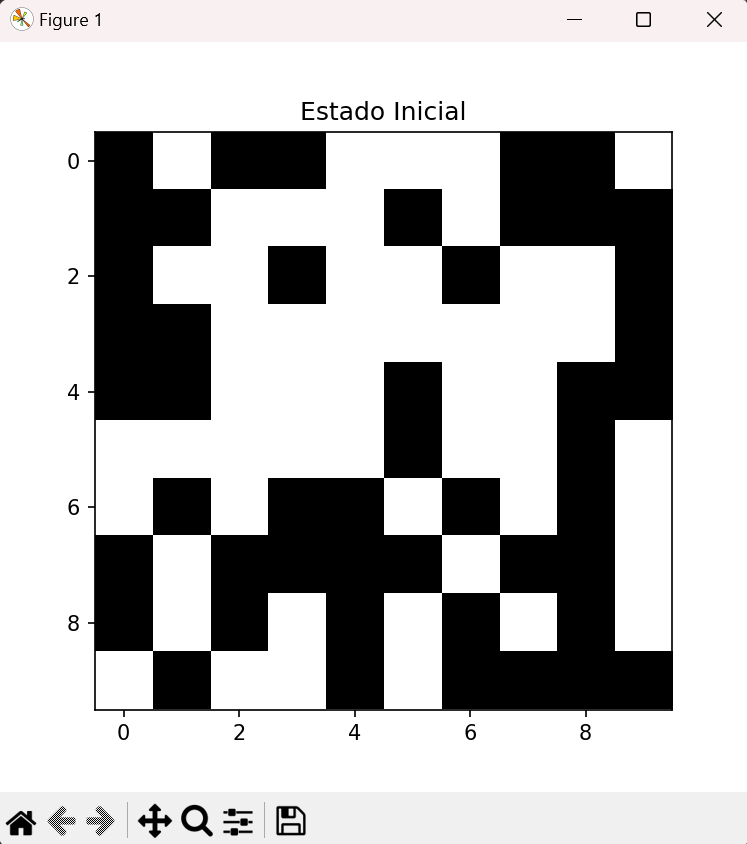
\includegraphics[scale=0.4]{Practica05/IMA/ejemplosJuegoVida/ejemplo 1.1.png}
    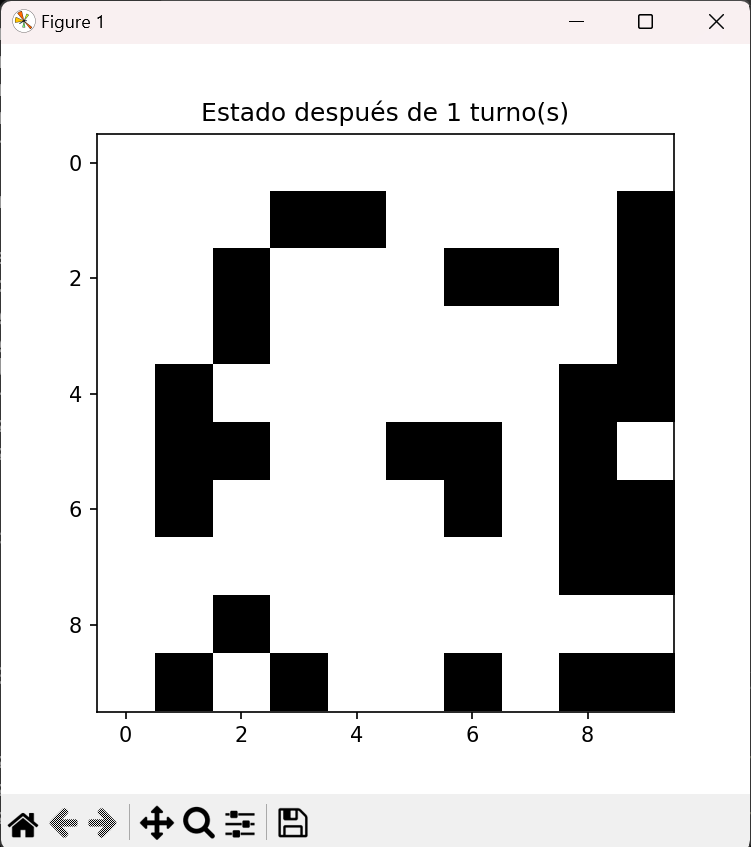
\includegraphics[scale=0.4]{Practica05/IMA/ejemplosJuegoVida/ejemplo 1.2.png}
    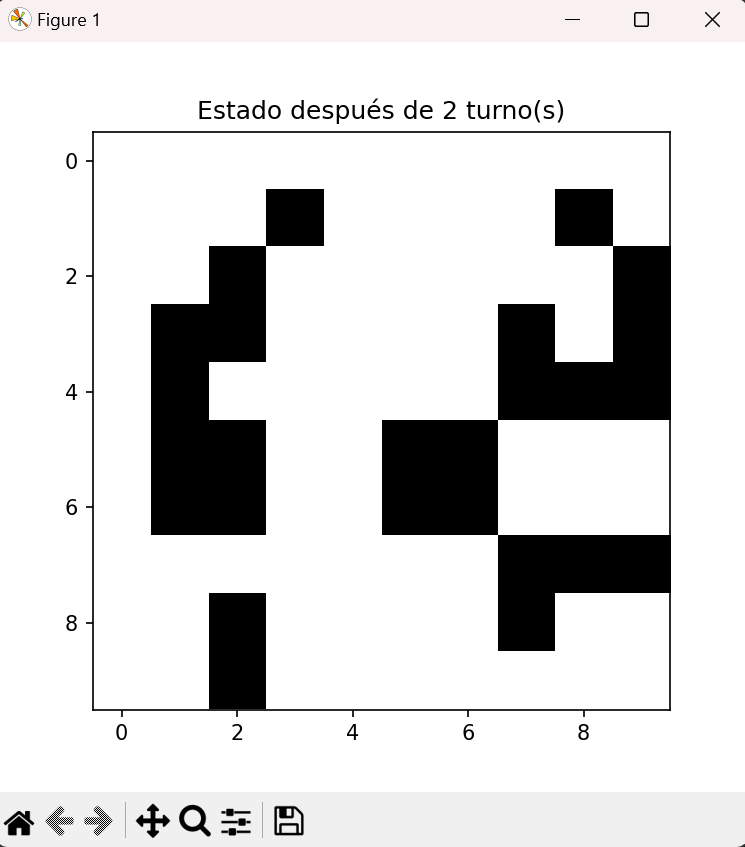
\includegraphics[scale=0.4]{Practica05/IMA/ejemplosJuegoVida/ejemplo 1.3.png}
    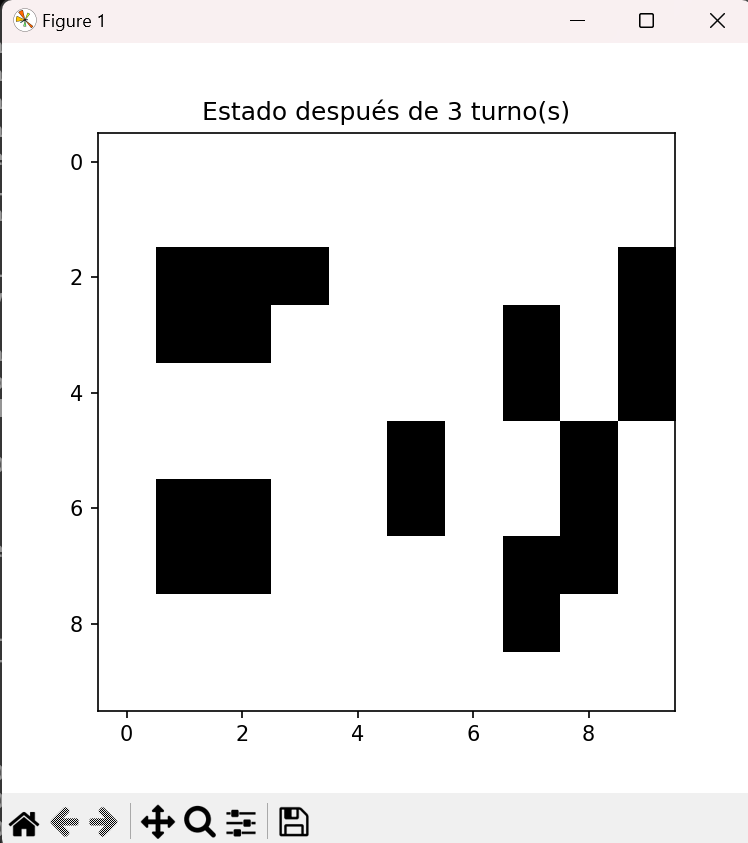
\includegraphics[scale=0.4]{Practica05/IMA/ejemplosJuegoVida/ejemplo 1.4.png}
    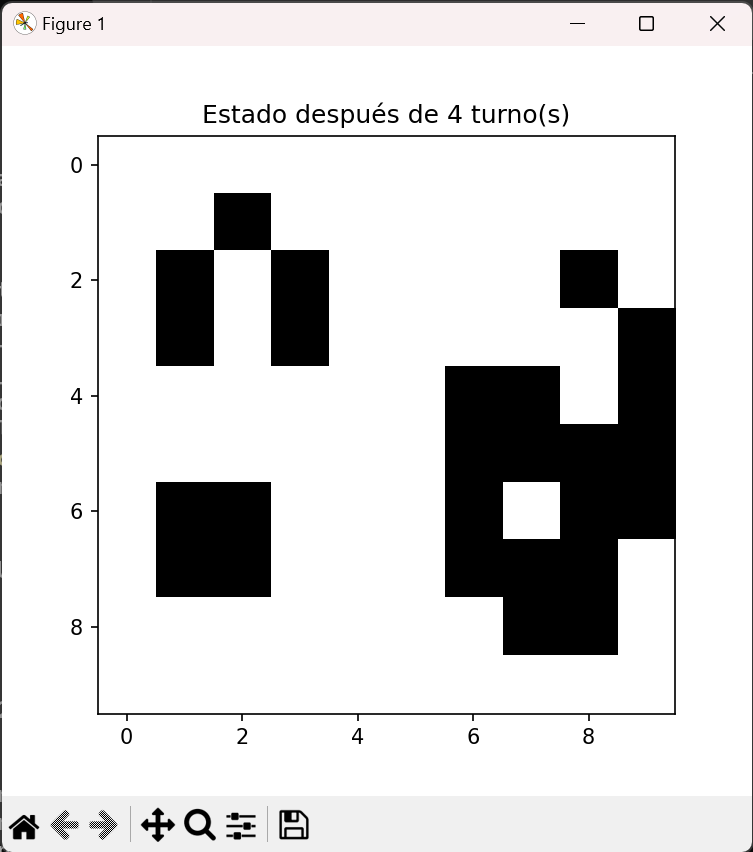
\includegraphics[scale=0.4]{Practica05/IMA/ejemplosJuegoVida/ejemplo 1.5.png}
    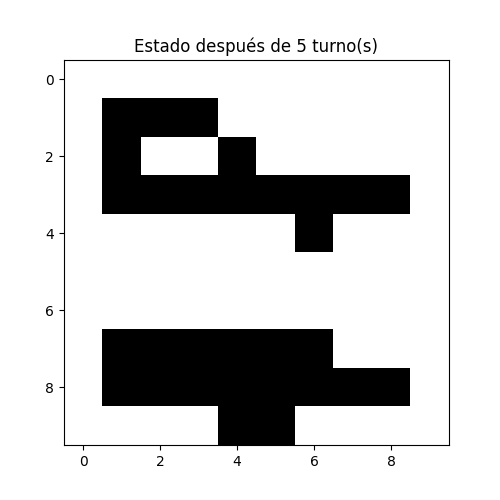
\includegraphics[scale=0.4]{Practica05/IMA/ejemplosJuegoVida/ejemplo 1.6.png}
\end{center}

    \item Estado inicial formado\\

\begin{lstlisting}
# Estado inicial formando un bloque estable
estado_actual = np.array([[0, 0, 0, 0, 0],
                           [0, 0, 1, 0, 0],
                           [0, 0, 1, 0, 0],
                           [0, 0, 1, 0, 0],
                           [0, 0, 0, 0, 0]]) 


# Visualizar el estado inicial
visualizar_estado(estado_actual, "Estado Inicial")

# Bucle para actualizar y visualizar el juego en cada turno
for i in range(num_iteraciones):
    # Aplicar las reglas del Juego de la Vida para obtener el nuevo estado
    estado_actual = aplicar_reglas(estado_actual)
    # Visualizar el estado actual después de aplicar las reglas
    visualizar_estado(estado_actual, titulo=f"Estado después de {i + 1} turno(s)")
\end{lstlisting}
    Los estados se muestran de la siguiente forma:
\begin{center}
    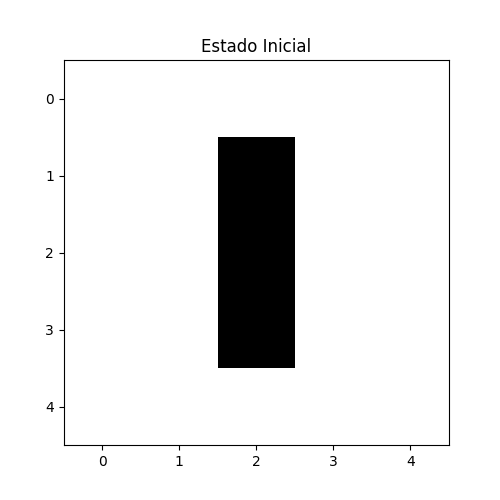
\includegraphics[scale=0.4]{Practica05/IMA/ejemplosJuegoVida/ejemplo 2.1.png}
    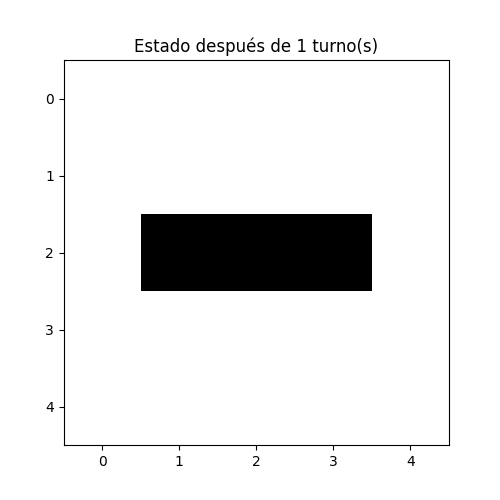
\includegraphics[scale=0.4]{Practica05/IMA/ejemplosJuegoVida/ejemplo 2.2.png}
    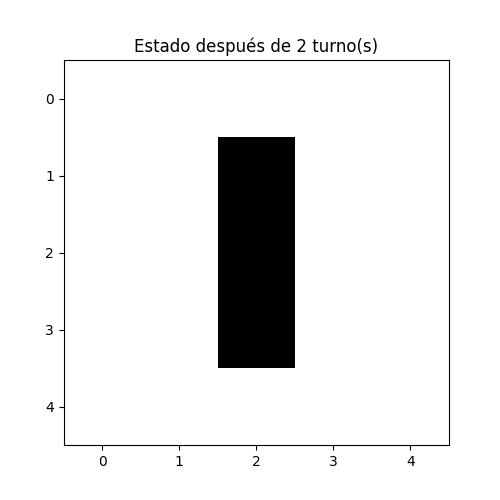
\includegraphics[scale=0.4]{Practica05/IMA/ejemplosJuegoVida/ejemplo 2.3.png}
    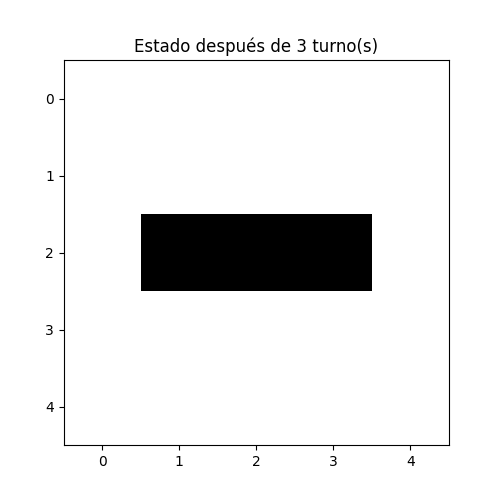
\includegraphics[scale=0.4]{Practica05/IMA/ejemplosJuegoVida/ejemplo 2.4.png}
    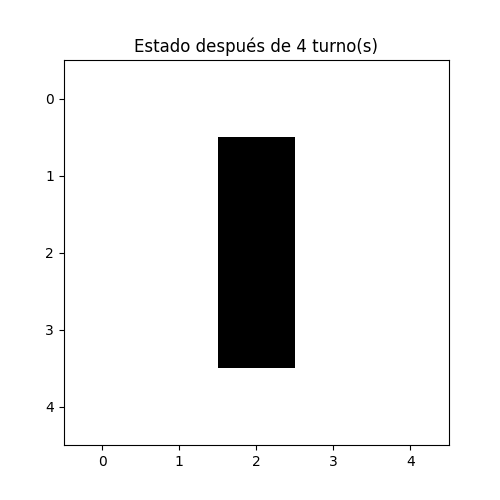
\includegraphics[scale=0.4]{Practica05/IMA/ejemplosJuegoVida/ejemplo 2.5.png}
    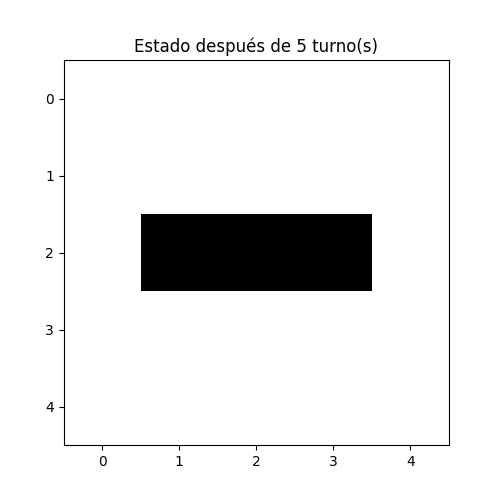
\includegraphics[scale=0.4]{Practica05/IMA/ejemplosJuegoVida/ejemplo 2.6.png}
\end{center}
    
\end{itemize}


%----------------------------------------------------------------------------------\    
    \item Introducción a los Algoritmos Genéticos
    \item Implementación de Algoritmos Genéticos en el Juego de la Vida
\end{enumerate}

% ----------------------------------------------------------------------------------------\
% ---------------------------------------------------------------------------------------\
% --------------------------------------------------------------------------------------\
\section{Investigación}
% ----------------------------------------------------------------------------------------\
% ---------------------------------------------------------------------------------------\
% --------------------------------------------------------------------------------------\

\subsubsection*{¿Qué es el algoritmo Genético?}

Un algoritmo genético \texttt{(AG)} entonces es: una técnica de resolución de problemas 
que utiliza principios inspirados en la selección natural para solucionar problemas de 
optimización. La selección natural (evolución) como estrategia implica la creación, 
reproducción y adaptación de una población de posibles soluciones en un rango de generaciones.\\ 

Este enfoque de población se basa en que cada individuo representa una posible solución 
al problema, y la evolución de estos comienza por, la \textbf{creación} de los individuos, 
la \textbf{reproducción} para después hacer la óptima \textbf{selección} de los padres en 
una nueva reproducción y \textbf{mutación}, finalmente comprobar o evaluar su \textbf{aptitud}\\ 


\subsubsection*{Pasos que sigue}

\begin{center}
    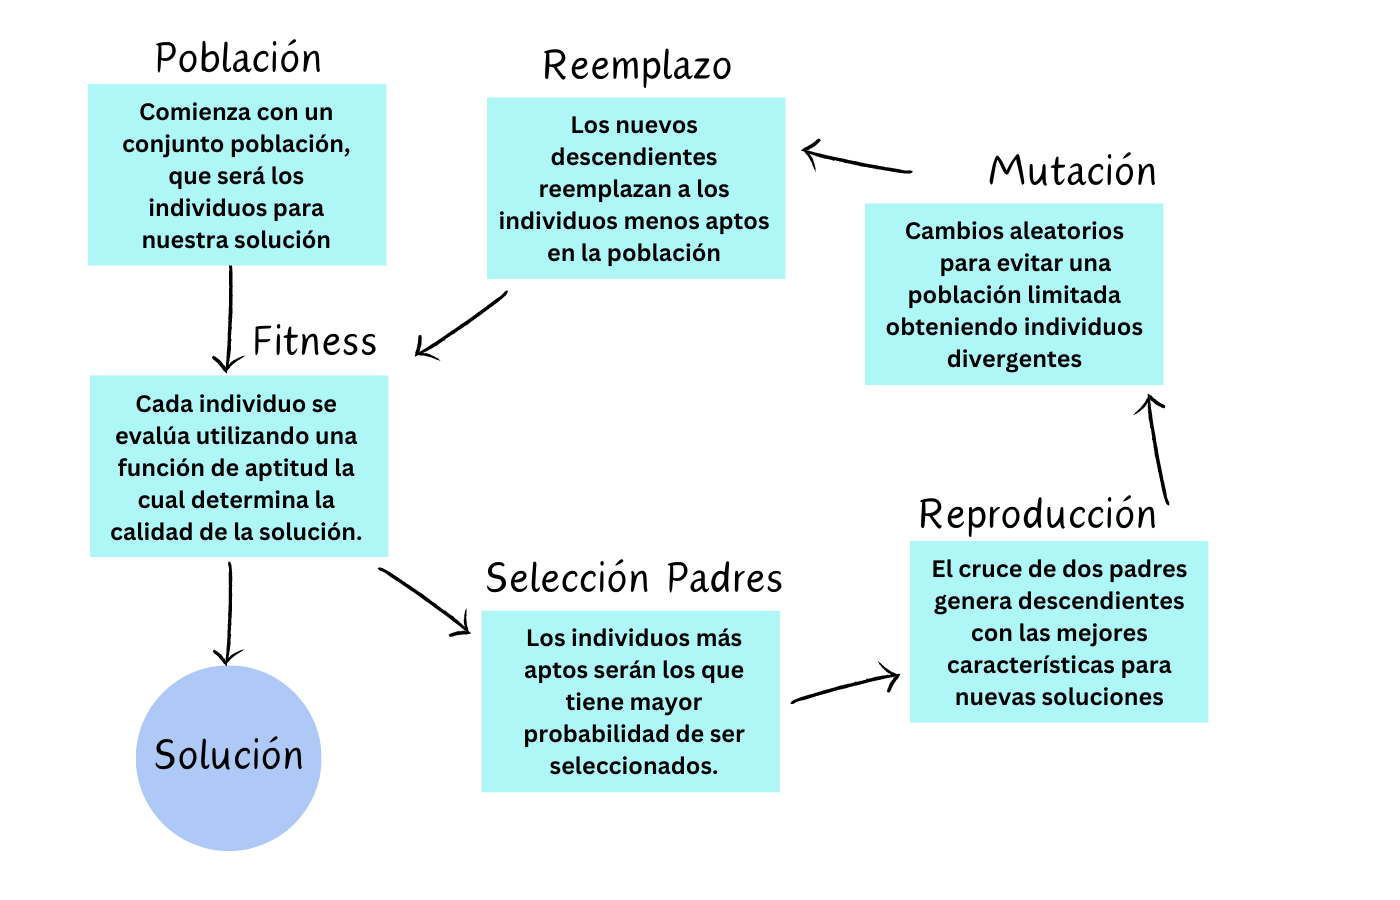
\includegraphics[scale = .4]{IMA/algo genetico.png}
\end{center}
